%encoding = utf-8
% Document information
% ====================
\title{Resumen Tésis MT4}
\author{Santiago Armstrong}
\date{\normalsize\today}


% Document configuration
% ======================

% Document Type, Font and paper size
\documentclass[12pt, letterpaper]{article}


% MT4 - header style
\usepackage{fancyhdr}

%References
\usepackage[notocbib]{apacite}

% Page Margins
\usepackage{fullpage}
\usepackage[left=2.5cm, right=2.5cm]{geometry}

% Text Margins
\setlength{\parindent}{0.5cm}
\renewcommand{\baselinestretch}{1.3}

% Font Type
\usepackage{times}

%% Languages
\usepackage[utf8]{inputenc}
\usepackage[british, spanish]{babel}

%% Basic imports
\usepackage{natbib}
\usepackage{graphicx}

%% Math imports
\usepackage{amsmath,amsthm,amssymb,amsfonts,mathrsfs,latexsym,stmaryrd}

%% Include PDF pages
\usepackage[final]{pdfpages}

%% Hyperlinks
\usepackage{url}
\usepackage[pdfborder={0 0 0}]{hyperref} % no border




\DeclareUnicodeCharacter{00A0}{ }


% TOC name
\addto\captionsspanish{
  \renewcommand{\contentsname}
    {Temario Tentativo}
}


% MT4 Page Numbering
\pagestyle{fancy}
\fancyhf{}
\usepackage{lastpage}
\rfoot{ \color{gray} \textit{Página \thepage } }



% MT4 - header style
\renewcommand{\headrulewidth}{0pt}
% \renewcommand{\footrulewidth}{0.1pt}
\voffset = -1.2cm
\topmargin = 0cm
\headheight= 40pt
\headsep = 0.5cm
\fancyhead[L]{ \color{gray}\begin{minipage}{\textwidth}\scshape \textit{Pontificia Universidad Cat\'olica de Chile\\
Dirección de Investigación, Innovación y Postgrado\\{Escuela de Ingeniería}} \end{minipage}}
\fancyhead[R]{\color{gray} \textit{MT4}}



% Document text
% =============
\begin{document}






% Primeras Páginas del documento (rellenar previamente y guardar en la carpeta docs)
% ----- 
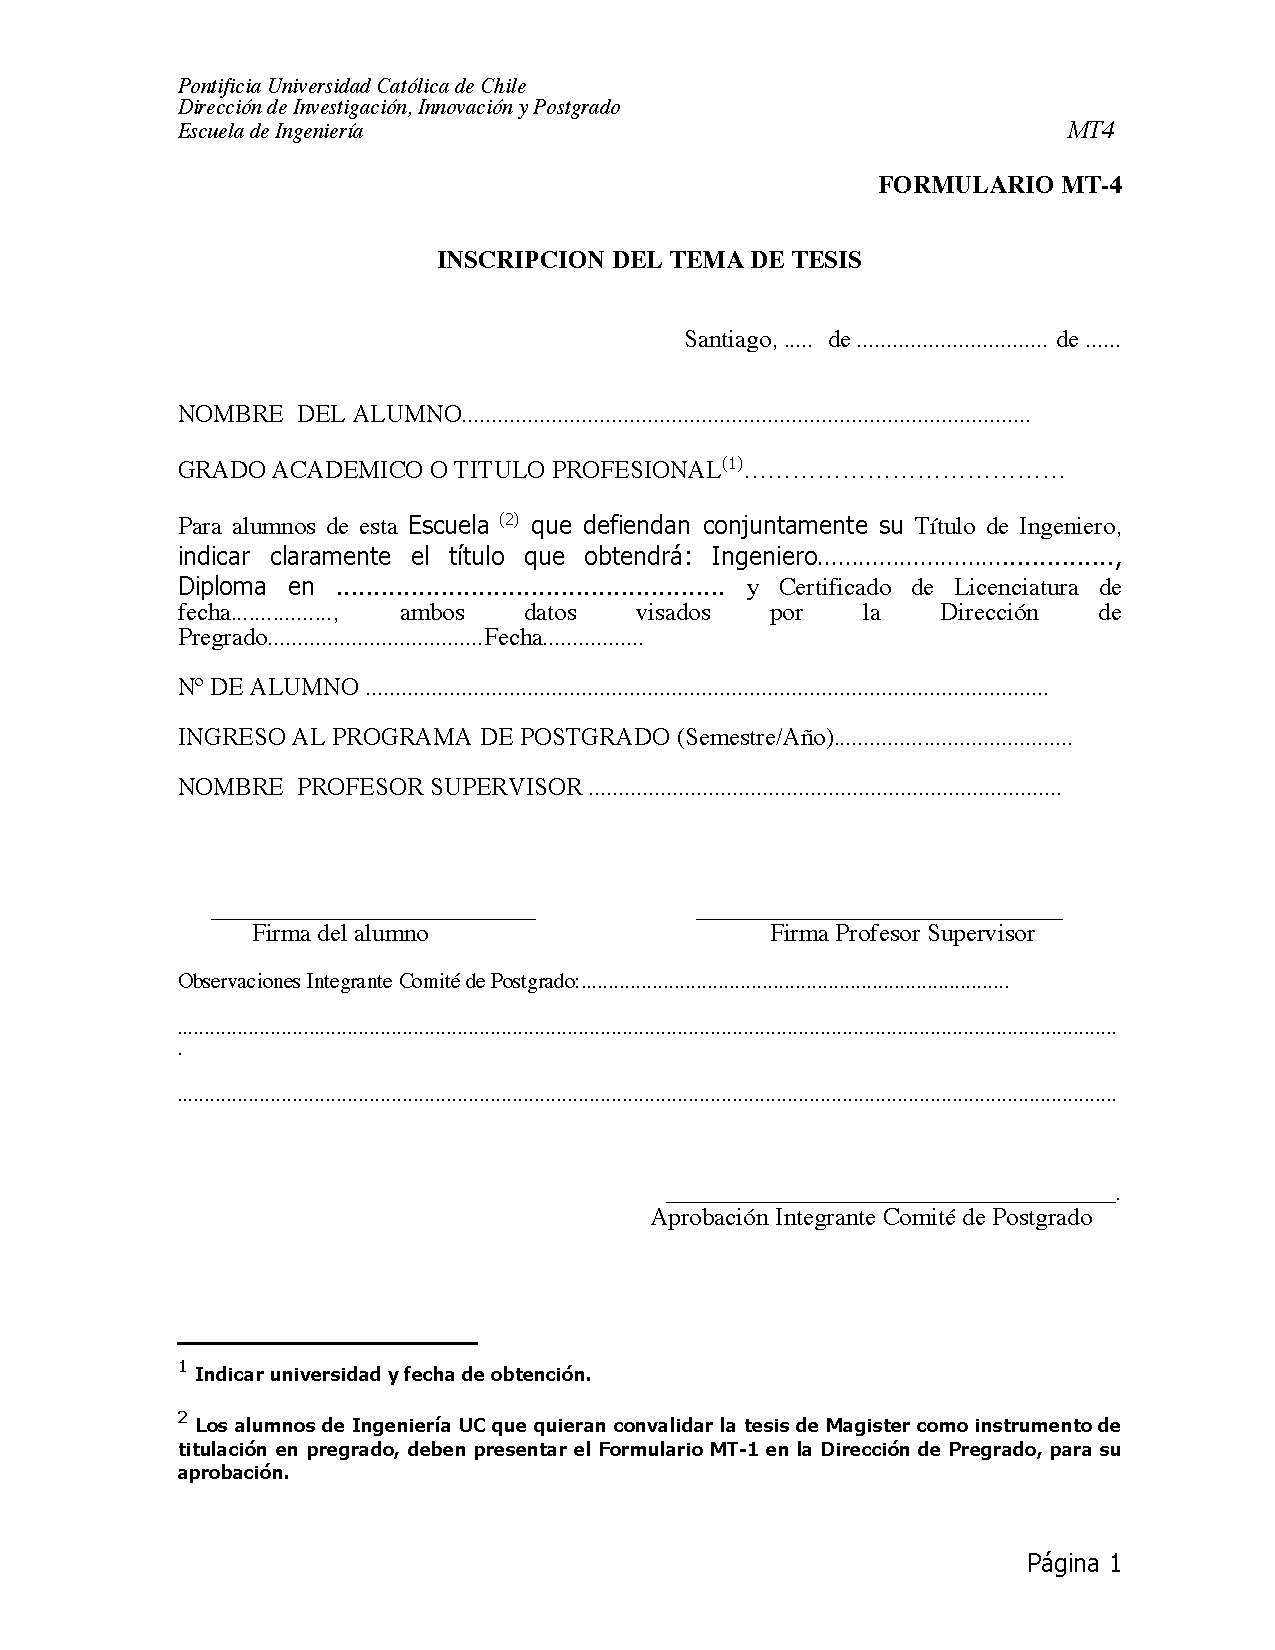
\includepdf[pages=-]{docs/FormularioMT4.pdf}


% Resumen
% -------
% Resumen Tesis
% ===============
\section*{Título de la Tesis}

\subsection*{Introducción}


La cristalización de lactosa ha sido ampliamente estudiada debido al interés que genera por su extendido uso en las industrias farmacéutica y alimentaria\cite{haase1966kinetic}


\subsection*{Hipótesis}

La hipótesis de este trabajo es que el desarrollo de una técnica de video-microscopía permite cuantificar con mayor precisión la cinética de cristalización de lactosa a partir de nucleación primaria heterogénea en comparación con técnicas tradicionales como la refractometría.











% References
% ----------
\bibliographystyle{apacite}
\bibliography{references}


% Indexes
% -------
% Content index stuff
% ===================

\tableofcontents

\section{Título}
\subsubsection{subtitle}

\section{Título}
\subsubsection{subtitle}





%\pagenumbering{arabic}% Arabic page numbers (and reset to 1)







\end{document}
